\section{Backgrounds}
\label{sect:bkg}
The backgrounds are studied in two categories: those with 
``misidentified'' \Tau, i.e., events where a quark or gluon jet has been misidentified
as a \Tau, and those with genuine \Tau candidates.
The QCD multijet and \wjets events are the dominant sources in the first category, while a mixture of \ttbar, Z+jets, diboson, and Higgs boson 
events dominate the second category. Background estimates are performed using control samples in data whenever possible. 
Those backgrounds that are taken from simulation are either validated in dedicated control regions or corrected using data-to-simulation scale factors. 
The estimates of the main backgrounds are discussed below, while the remaining contributions are small and are taken from simulation.


\subsection{\texorpdfstring{The QCD multijet background estimation in the \tauTau channel}{The QCD multijet background estimation in the tau-tau channel}}
\label{sect:bkgQCD}
Events from QCD multijet production can appear in the signal regions if two hadronic jets are misidentified as a \tauTau pair.
The isolation variable is a powerful discriminant between misidentified and genuine \Tau candidates. To estimate the QCD multijet contribution, an ABCD method is used, where three \tauTau control regions (CRs) are defined using the loose \Tau isolation requirement, together with lower thresholds on \mttwo or \SumMT variables for the corresponding signal region. The former is changed from \mttwo $>$ 90 to $>$ 40\GeV, whereas the latter is reduced from \SumMT $>$ 250 to $>$ 100\GeV. In addition, the requirement on \deltaphi is removed to increase the number of events in the CRs. 
To reduce contamination from genuine \tauTau events 
in CRs with at least one loose \Tau candidate, 
same-sign (SS) \tauTau pairs are selected. Residual contributions from genuine 
\tauTau and \wjets events (non-QCD events) are subtracted based on MC expectations. 
The CR and signal region are illustrated in Fig.~\ref{fig:ABCDQCD}. 
\begin{figure}[!htb]
\centering
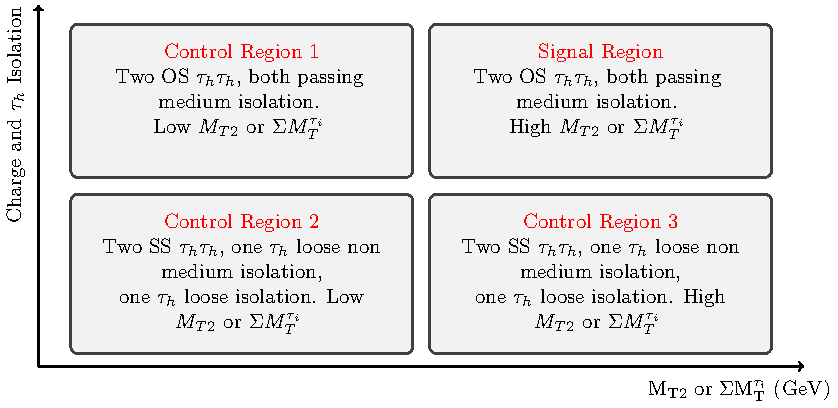
\includegraphics[angle=0,scale=1.15]{Bkg/ABCD.pdf}
\caption{Schematic illustration of three control regions and the signal region used to estimate the QCD multijet background.}
\label{fig:ABCDQCD}
\end{figure}
In the samples dominated by QCD multijet events (CR1 and CR2), the isolation of misidentified \Tau candidates is verified 
to be almost completely uncorrelated with the search variables \mttwo and \SumMT.
The QCD multijet background in the signal regions is therefore estimated by scaling the number of QCD multijet events with high \mttwo or high \SumMT and loosely isolated SS \tauTau (CR3) by a transfer factor, 
which is the $y$-intercept of a horizontal line fitted to the ratio of the numbers of events in CR1 and CR2 in different bins of the 
low values of the search variables.
The final estimate of the background is corrected for the efficiency of 
the \deltaphi requirement for QCD multijet events. This efficiency is measured in CR1 and CR2, 
in which the contribution of QCD multijet events is more than $80\%$. It is checked that the efficiency versus the search variable is 
same in both CR1 and CR2 and to gain in statistics, two CRs are combined before measuring the efficiency. 
The efficiency is a falling distribution as a function of 
the search variable (\mttwo or \SumMT) and the value of the last bin ($65<\mttwo<90\GeV$ or $200<\SumMT<250\GeV$) 
is used conservatively as the value of the efficiency in the signal regions.

The number of data events in CR3 after subtracting the non-QCD events is 4.81 $\pm$ 2.57 (8.62 $\pm$ 3.55) for the \binone (\bintwo) selection.
For SR1 (SR2), the transfer factors and  \deltaphi efficiencies are measured to be 0.91 $\pm$ 0.12 (0.89 $\pm$ 0.11) and 0.03 $^{+0.04} _{-0.03}$ (0.15 $\pm$ 0.08), 
respectively.
The reported uncertainties are the quadratic sum of the statistical and systematic uncertainties.


The systematic uncertainty in the background estimates includes the uncertainty in the validity of the assumption that isolation 
and \mttwo or \SumMT are not correlated, the \deltaphi efficiency is extrapolated correctly to the signal regions, and the uncertainties in the residual 
non-QCD SM backgrounds which  are subtracted based on MC expectations for different components of the background estimation. 
The latter includes both the statistical uncertainty of the simulated 
events and also a 22\% systematic uncertainty that will be discussed in Section~\ref{sect:sys}, 
assigned uniformly to all simulated events.

 
Table \ref{4QCDbg} summarizes the estimation of the QCD multijet background contribution in the two signal regions after extrapolation from 
the control regions and correcting for the \deltaphi efficiency. 
To evaluate the uncertainties in the transfer factor and \deltaphi efficiency due to the correlation assumptions, 
different fit models are tested. 
Fitting the whole range of the low values of the search variables by a horizontal line or a line with a constant slope 
or using the value of the last bin before entering the signal region are examined. 
The weighted average of the estimates is compared with the reported values 
in Table \ref{4QCDbg} to extract the ``fit'' uncertainty.
\begin{table}[!htb]
\begin{center}
\caption{The estimated QCD multijet background event yields in the \tauTau channel. The first two uncertainties are the statistical and systematic uncertainties of the method, and the last uncertainty is the extra systematic uncertainty due to the correlation assumptions.}
\begin{tabular}{|l|c|}
\hline
 Signal region       & QCD multijet  background estimate\\
\hline\hline
\tauTau \binone      & 0.13 $\pm$ 0.06 (stat) $^{+0.18} _{-0.13}$ (syst) $\pm$ 0.10 (fit) \\
\tauTau \bintwo      & 1.15 $\pm$ 0.39 (stat) $\pm$ 0.70 (syst) $\pm$ 0.25 (fit) \\
\hline
\end{tabular}
\label{4QCDbg}
\end{center}
\end{table}

\subsection{\texorpdfstring{\wjets background estimation in the \tauTau channel}{W+jets background estimation in the tau-tau channel}}
\label{sect:bkgW}
In the \tauTau channel, the number of remaining events for \wjets from MC is zero,
but it has a large statistical uncertainty due to the lack of the statistics in the simulated sample. To
have a better estimation, the contribution of the \wjets background in the \tauTau channel is taken from simulated events, using the formula:
\begin{equation}
N_{\rm SR} = \epsilon_{\rm{FS}}N_{\rm BFS} .
\end{equation}
Here $N_{\rm SR}$ is the estimation of \wjets events in the signal region, $N_{\rm BFS}$ is the number of 
\wjets events before applying the final selection criterion (\mttwo $>$ 90\GeV for \binone and \SumMT $>$ 250\GeV for \bintwo), but after applying all other selection criteria, including \mttwo $>$ 40\GeV for \binone and 40 $<\mttwo<$ 90\GeV for \bintwo.
The efficiency of the final selection ($\epsilon_{\rm{FS}}$) is defined as $\frac{N (\rm M_{T2}>90)}{N (\rm M_{T2}>40)}$ for \binone and $\frac{N (\SumMT>250)}{N(40<\rm M_{T2}<90)}$ for \bintwo.
The value of $N_{\rm BFS}$ is 31.9$\pm$6.4 (29.1$\pm$6.2) for \binone (\bintwo), where the uncertainties arise from the limited number of simulated events. 


The $\epsilon_{\rm{FS}}$ is evaluated in a simulated \wjets sample with a pair of opposite-sign \Tau candidates, where the \Tau candidates 
are selected with the same identification requirements as in the signal region, but with looser kinematic selection criteria to improve statistical precision.
Additional signal selection requirements on \deltaphi or the lepton veto are applied one by one such that two orthogonal subsamples (passing and failing) are obtained. The $\epsilon_{\rm{FS}}$ quantity is calculated in all subsamples. 
The values are consistent with those obtained from the sample defined with relaxed requirements 
within the statistical uncertainties. 
The measured $\epsilon_{\rm{FS}}$ values from the looser-selection samples are  
0.028 $\pm$ 0.010 and 0.098 $\pm$ 0.032 for \binone and \bintwo, respectively.
The uncertainty in the \Tau energy scale is also taken  into account in the uncertainty in $\epsilon_{\rm{FS}}$.


The \wjets simulated sample is validated in data using a same-sign \muTau control sample, where both the normalization and $\epsilon_{\rm{FS}}$ are checked. 
The ratio of data to MC expectation is found to be 1.05 $\pm$ 0.13 (1.02 $\pm$ 0.09) for \binone(\bintwo), 
which is compatible with unity within the uncertainties. 
For $\epsilon_{\rm{FS}}$, to take into account the difference between the data and MC values, 
the MC prediction in each of the two signal regions is corrected by the ratio of $\epsilon_{\rm FS(data)}$ to $\epsilon_{\rm FS(MC)}$, 
which is 0.73 $\pm$ 0.57 (1.49 $\pm$ 0.38) for \binone(\bintwo), and its uncertainty is also taken to be the ``shape'' systematic uncertainty.

Table \ref{tbl:Wbkg} summarizes the estimated results for different signal regions for the \tauTau channel.
\begin{table}[!htb]
\begin{center}
\caption{The \wjets background estimate in the two search regions. 
The systematic uncertainty ``syst'' comes from the maximum
variation of the estimation found  from varying the \Tau energy scale within its uncertainty. 
The ``shape'' uncertainty takes into account the difference between the shape of the search variable distribution in data and simulation.}
\begin{tabular}{|l|c|}
\hline
Signal Region & \wjets background estimate\\
\hline\hline
\tauTau \binone & 0.70 $\pm$ 0.21 (stat) $\pm$ 0.09 (syst) $\pm$ 0.54 (shape)\\
\tauTau \bintwo & 4.36 $\pm$ 1.05 (stat) $\pm$ 1.14 (syst) $\pm$ 1.16 (shape)\\
\hline
\end{tabular}
\label{tbl:Wbkg}
\end{center}
\end{table}

\subsection{The Drell--Yan background estimation}
The DY background yield is obtained from the MC simulation. 
The simulated sample includes production of different lepton pairs ($\rm{ee}$, $\mu\mu$, and $\tau\tau$). 
The contribution from \Z$\rightarrow \ell \ell$ and \Z$\rightarrow \tau \tau\rightarrow \ell \ell$ events is found to be very small, because the misidentification probabilities for $\ell\rightarrow$  \Tau are sufficiently low.  
The dominant background events are \Z$\rightarrow \tau \tau\rightarrow \ell \Tau$ and \Z$\rightarrow \tau \tau\rightarrow \Tau \Tau$ decays.
The misidentification probability for  \Tau $\rightarrow\ell$ is also low, so the probability 
to have DY background contribution from \Z$\rightarrow \tau \tau\rightarrow \Tau \Tau$ events in the \leptonTau channels is negligible.
The simulation is validated in a \muTau control region obtained by removing the \deltaphi
requirement and by inverting the \Z boson veto and also by requiring \mttwo $<$ 20\GeV,  40 $<$ \tauMT $<$ 100\GeV.  
The distributions of the invariant mass of the \muTau system for data and simulated events are in good agreement.
The \PT of the \Z boson system, which is correlated with 
\mttwo, is also well reproduced in simulation. Table \ref{tbl:DYbkg}
summarizes the DY background contribution in the different signal regions. 
For \leptonTau channels, only the contributions from the genuine lepton+\Tau are reported. 
A separate method is developed in Section~\ref{sect:bkgFake} to estimate the misidentified lepton contamination in these channels.
\begin{table}[!htb]
\begin{center}
\caption{The DY background contribution estimated from simulation in four signal regions.  The uncertainties are due to the limited number of MC events.}
\begin{tabular}{|l|c|}
\hline
Signal Region      &  DY background estimate\\
\hline\hline
\eTau              & 0.19  $\pm$  0.04\\\hline%  $\pm$ 0.05 \\\hline
\muTau             & 0.25  $\pm$  0.06\\\hline%  $\pm$ 0.07 \\\hline
\tauTau \binone    & 0.56  $\pm$  0.07\\\hline%  $\pm$ 0.16 \\\hline
\tauTau \bintwo    & 0.81  $\pm$  0.56\\\hline%  $\pm$ 0.23 \\
\end{tabular}
\label{tbl:DYbkg}
\end{center}
\end{table}


\subsection{\texorpdfstring{Misidentified \Tau in the \leptonTau channels}{Misidentified tau in the lepton-tau channels}}
\label{sect:bkgFake}
The contribution from misidentified \Tau in the \leptonTau channels is estimated using a method which takes into account the probability 
that a loosely isolated misidentified or genuine \Tau passes the tight isolation requirements.
If the signal selection is done using the \Tau candidates that pass the loose isolation, 
the number of loose \Tau candidates ($N_{\rm l}$) is:

\begin{equation}
N_{\rm l} = N_{\rm g} + N_{\rm m}
\end{equation}
where $N_{\rm g}$ is the number of genuine \Tau candidates and $N_{\rm m}$ is the number of misidentified 
\Tau candidates. If the selection is tightened, the number of tight \Tau candidates ($N_{\rm t}$)  is

\begin{equation}
 N_{\rm t} = r_{\rm g} N_{\rm g} + r_{\rm m} N_{\rm m}
\end{equation} 
where $r_{\rm g}$ ($r_{\rm m}$) is the genuine (misidentified \Tau) rate, i.e., the probability that a loosely selected genuine (misidentified) \Tau candidate passes the  tight  selection. 
One can obtain the following expression by eliminating $N_{\rm g}$:

\begin{equation}
   r_{\rm m} N_{\rm m}  = r_{\rm m} (N_{\rm t} - r_{\rm g} N_{\rm l})/(r_{\rm m}-r_{\rm g}).
\end{equation}
Here, the product $r_{\rm m} N_{\rm m}$ is the contamination of misidentified \Tau candidates in the signal region. 

The misidentification rate ($r_{\rm m}$) is measured as the ratio of tightly selected \Tau candidates to loosely 
selected \Tau candidates in a sample dominated by misidentified \Tau candidates. 
This is done in a data sample with the same selection as \leptonTau, except with an inverted
\MPT requirement, i.e., \MPT $<$ 30\GeV. The misidentification rate is measured to be 0.54 $\pm$ 0.01.
The genuine \Tau candidate rate ($r_{\rm g}$) is estimated in simulated DY events; it is found to 
be $r_{\rm g}$ = 0.766 $\pm$ 0.003 and almost independent of \mttwo. 
A relative systematic uncertainty of 5\% is assigned to the central value of $r_{\rm g}$ to cover its 
variations for different values of \mttwo.
The method is validated in the simulated \wjets sample using the misidentification rate which is evaluated with the same method as used for data. 
%The result is compared to the case where $r_{\rm m}$ = 0.54 is used. 
%To cover the differences, a 5\% relative systematic uncertainty is
%assigned to the central values of the misidentification rates.
This misidentification rate is $r_{\rm m}$ = 0.51. 
%which has a 5\% relative difference with $r_{\rm m}$ = 0.54. 
This difference is taken as the systematic uncertainty of 5\% 
%which is a 5\% relative uncertainty.
in the central value of the misidentification rate ($r_{\rm m}$ = 0.54).
The method predicts the number of \leptonTau background events in this sample within the 
uncertainties.
These include statistical uncertainties due to the number of events in the 
sidebands (loosely selected \Tau candidates), as well as 
systematic uncertainties.
The uncertainties in the 
misidentification rate and the genuine \Tau candidate rate 
are negligible compared to the statistical uncertainties associated to 
the control regions. 

The estimates of the misidentified \Tau contamination in the two \leptonTau 
channels are summarized in Table~\ref{Tab.FakeEstimation}. 
The relative statistical and systematic uncertainties are reported separately. 
Since the same misidentified and genuine \Tau candidate rates are used to estimate the backgrounds for both
\eTau and \muTau channels, the total systematic uncertainties have to be considered 
fully correlated between the two channels.
\begin{table}[!htb]
\begin{center}
\caption{Estimation of the misidentified \Tau contribution in the signal region of the \leptonTau channels. The total systematic uncertainty is the
quadratic sum of the individual components. All uncertainties are relative.
The $r_{\rm m}$ ($r_{\rm g}$) is shorthand for misidentified (genuine) \Tau candidate rate.}
\begin{tabular}{|l|c|c|c|c|c|}
\hline
Channel    & Total misid (events) & Stat (\%) &  $r_{\rm m}$ syst (\%) & $r_{\rm g}$  syst (\%) & Total uncert (\%) \\\hline\hline
\eTau      &   3.30     &  101    &  17    & 2  & 102  \\
\muTau     &   8.15     &   56    &  18    & 5   & 59  \\
\hline
\end{tabular}
\label{Tab.FakeEstimation}
\end{center}
\end{table}
